\subsection{Modelado}

\subsection{Modelado Del Juego}

El juego en si consistirá en una lista de listas donde cada lista representará una columna del tablero. En cada turno un jugador elegirá una columna numerada del 0 al n, siendo n el numero de columnas totales y el juego se encargará. Ambos jugadores contarán en el momento de la elección con el estado actual del tablero.

Luego de cada jugada, el juego chequeará si el jugador ganó o si ya no hay mas movimientos posibles, terminando el juego e informando que jugador gano o si fue empate.

El pseudocódigo del juego será, entonces el siguiente:

\begin{algorithm}[h!]
\begin{algorithmic}[1]\parskip=1mm
 \caption{jugar()}
 \STATE{While True}
 \STATE{\quad columna = player.move(tablero)}
 \STATE{\quad jugar\_ficha(columna, tablero)}
 \STATE{\quad if jugador\_gano(tablero)}
 \STATE{\quad\quad return player}
 \STATE{\quad if tablero\_lleno(tablero)}
 \STATE{\quad\quad return empate}
 \STATE{\quad player = otro\_jugador(player)}
\end{algorithmic}
\end{algorithm}

Como ya adelantamos en la introducción, es necesario definir en que etapa del algoritmo se le asignará la recompensa al algoritmo de q-learning. Una opción bastante sencilla e intuitiva es la de asignar recompensas en el momento en que algún jugador gana la partida. Por ejemplo al ganar la partida uno de los jugadores, se le asigna una recompensa de $1$ a el y una recompensa de $-1$ al contrincante. Siguiendo con el lineamiento anterior, también sería posible asignarles recompensas en el momento en que se empata, por ejemplo, asignándoles a ambos jugadores una recompensa de $0.5$

En caso de que no se haya llegado a un estado final, una posible propuesta es asignarle al otro jugador una recompensa por ejemplo de 0.

El pseudocódigo entonces, pasaría a verse de la siguiente manera:

\begin{algorithm}[h!]
\begin{algorithmic}[1]\parskip=1mm
 \caption{jugar()}
 \STATE{While True}
 \STATE{\quad columna = player.move(tablero)}
 \STATE{\quad jugar\_ficha(columna, tablero)}
 \STATE{\quad if jugador\_gano(tablero)}
 \STATE{\quad\quad player.recompensa(1)}
 \STATE{\quad\quad otro\_jugador(player).recompensa(-1)}
 \STATE{\quad\quad return player}
 \STATE{\quad if tablero\_lleno(tablero)}
 \STATE{\quad\quad player.recompensa(0.5)}
 \STATE{\quad\quad otro\_jugador(player).recompensa(0.5)}
 \STATE{\quad\quad return empate}
 \STATE{\quad otro\_jugador(player).recompensa(0)}
 \STATE{\quad player = otro\_jugador(player)}
\end{algorithmic}
\end{algorithm}


\subsection{Modelado De Jugadores}

Un jugador estará compuesto por dos métodos básicos, uno que llamaremos $move()$ que, dado un estado del tablero devuelve una acción valida (tirar ficha en la primera columna, en la segunda, etc) y una función $reward()$ que nos dirá en que estado quedo el juego luego de movernos y de que el oponente moviera y una recompensa que utilizaremos para actualizar la matriz $Q$ en caso de que el jugador lo requiera.

En particular, para la clase jugador que implemente q-learning el algoritmo para decidir que acción realizar vendrá dado de la siguiente manera:

\begin{algorithm}[h!]
\begin{algorithmic}[1]\parskip=1mm
 \caption{move(tablero)}
 \STATE{acciones\_validas = elegir\_acciones\_validas(tablero)}
 \STATE{Para cada acción en acciones\_validas}
 \STATE{\quad obtener q para accion}
 \STATE{\quad guardarlo en lista de qs\_validos}
 \STATE{accion\_elegida = elegir\_acción(acciones\_validas,qs\_validos)}
 \STATE{retornar accion\_elegida}
\end{algorithmic}
\end{algorithm}

Y la función learn, que básicamente consiste en adaptar la función de aprendizaje vista en la teórica:

\begin{algorithm}[h!]
\begin{algorithmic}[1]\parskip=1mm
 \caption{learn(tablero,recomensa)}
 \STATE{prev\_q = getQ(estado\_previo, accion\_elegida)}
 \STATE{maxqnew = tomar maximo q de tomar una acción en el tablero resultante}
 \STATE{q[(estado\_previo, accion\_elegida)] = prev + $\alpha$ * ((reward + $\gamma$*maxqnew) - prev)}
\end{algorithmic}
\end{algorithm}

Aquí quedan por definir varios parámetros, entre ellos $\alpha$, $\gamma$ y los valores iniciales para la matriz $Q$. En primera instancia decidimos tomar valores que Consideramos apropiados de a cuerdo a datos empíricos de la implementación y que consideramos razonables. Tomaremos $\alpha=0.4 $, $\gamma=0.9$ y todas los valores de Q iniciarán con $1$ con el objetivo de alentar la exploración.

En la siguiente sección propondremos distintos algoritmos para elegir una acción tomado del jugador y teorizar como estas impactan en el aprendizaje.

\subsection{Planteo De Distintas Estrategias de Movimiento}

En esta sección plantearemos distintas estrategias que utilizará nuestro jugador al momento de elegir si explorar nuevas posibilidades o utilizar el mejor camino conocido.

La primera estrategia que plantearemos es una estrategia greedy en donde el jugador tomara un camino random con probabilidad $\epsilon\%$ y en caso contrario utilice el mejor brazo conocido.

La segunda estrategia es conocida como $\epsilon$-first: en este caso el jugador toma un camino random en las primeras $\epsilon$ iteraciones y luego toma el mejor camino conocido.

Como ultima estrategia utilizaremos Softmax: basada en una función probabilística, la estrategia Softmax se basa en darle probabilidades distintas a cada acción posible dependiendo de la recompensa esperada de cada una de ellas.

En particular la probabilidad de cada una de las acciones vendrá dada por:

$$P_t(a) = \frac{\exp(q_t(a)/\tau)}{\sum_{i=1}^n\exp(q_t(i)/\tau)}$$

Donde $q_t(a)$ es el valor del valor esperado siguiendo la acción $a$ y la variable $\tau$ se denomina parámetro de temperatura, para temperaturas cercanas a infinito todas las acciones tienen aproximadamente la misma probabilidad de ser elegidas, mientras que para temperaturas bajas (cercanas a cero) la probabilidad de la acción de mayor recompensa tenderá a $1$.

En particular nuestra estrategia consistirá en comenzar con una temperatura alta para favorecer la exploración e ir gradualmente disminuyéndola para favorecer mas a aquellas con mayor recompensa. Faltará definir de alguna manera cual será el valor inicial de $\tau$ y de que manera reduciremos su valor (algunas posibilidades son de manera linea, logarítmica, etc).

\subsection{Análisis Espacio De Estados}

Según el modelo planteado para la resolución del problema, la matriz Q tendrá como como columnas los diferentes estados en los que se puede encontrar el tablero y como filas las acciones que se pueden realizar sobre ese determinado tablero. Dado que la cantidad de estados diferentes en los que se puede encontrar el tablero tiene complejidad PSPACE y que la cantidad la acciones es acotada (a lo sumo m), podemos determinar que la complejidad espacial de nuestro algoritmo esta en PSPACE... not cool.

Si bien esto hace que la complejidad de explorar cada una de las posibilidades sea extremadamente costosa, consideramos que para la mayoría de los casos no es necesario conocer todo el árbol sino los estados mas generales.

%referencia http://www.tzi.de/~edelkamp/publications/conf/ki/EdelkampK08-1.pdf


\pagebreak
\section{Experimentación}

\section{Estrategias vs Jugador Random}

Como primera instancia en la etapa de experimentación, haremos competir a un jugador q-learner contra un jugador que elige entre los posibles movimientos con probabilidad uniforme. Utilizaremos las tres estrategias enunciadas previamente para ver como se comporta cada una. 

La metodología utilizada para observar como evoluciona el algoritmo de q-learning será la de hacer jugar a ambos jugadores $10000$ veces randomizando cual es el que comienza primero. Luego tomaremos estos resultados y cada $250$ juegos, graficaremos cuantas veces ganó el algoritmo q-learning. 

Para la estrategia greedy, eligiendo un $\epsilon=0.1$ obtuvimos los siguientes resultados:

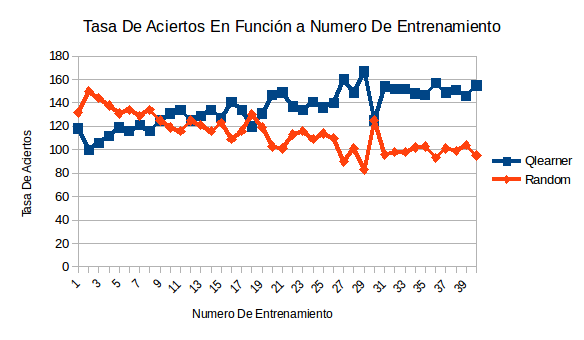
\includegraphics[scale=0.5]{testing/greedy.png}

%concluciones

Para la estrategia $\epsilon$-first eligiendo un $\epsilon=10\%$, y los resultados fueron los siguientes:

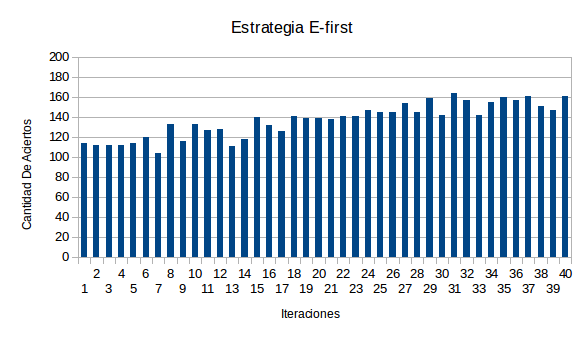
\includegraphics[scale=0.5]{testing/ef.png}

Puede verse como en el primer $10\%$ de las iteraciones el algoritmo gana la mitad de las veces y pierde la otra mitad, lo que era de esperarse para una política completamente random.

Con la tercera política Soft-Max, decidimos utilizar una temperatura inicial igual a $1$ y una función de calor que decirse de manera logarítmica con cada iteración:

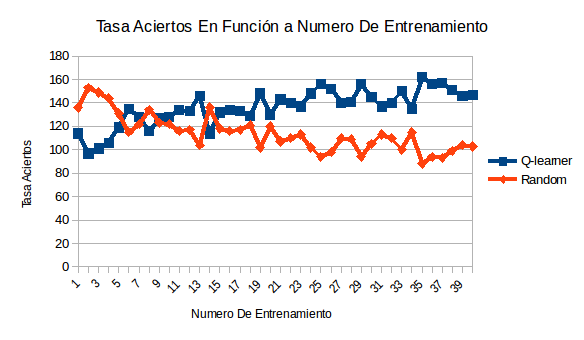
\includegraphics[scale=0.5]{testing/softmax.png}

%concluciones

\subsection{Performance de dos q-learners compitiendo}

En esta sección analizaremos el comportamiento de dos jugadores q learners (ambos utilizando una estrategia e-first) compitiendo entre si y aprendiendo al mismo tiempo. Lo que esperamos observar es que tras un periodo de tiempo donde ambos jugadores obtienen una tasa de aciertos cercano al $50 \%$ esta taza empiece converger a un numero mas bajo a medida que ambos converjan a una misma estrategia ganadora. Los resultados obtenidos fueron los siguientes:

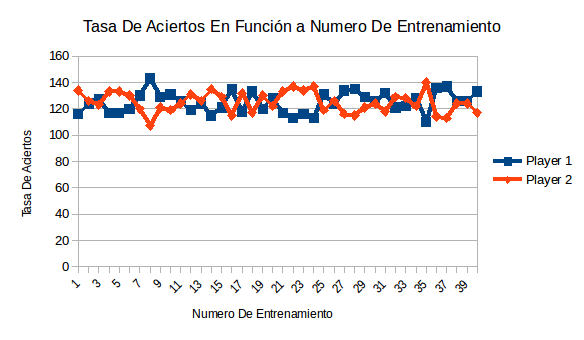
\includegraphics[scale=0.5]{testing/qvsq.png}

Se realizó la misma experimentación con las otras dos estrategias obteniéndose resultados similares en ambos casos. Esto aproxima a los valores esperados, una hipótesis posible es que el jugador que juega primero tenga mas ventaja que el que juega segundo y por lo tanto, al estar randomizado el orden en que empiezan, la mitad de las veces gane uno y la otra mitad gane el otro. Para testear esto modificamos el programa para que el jugador 1 siempre comience primero y el jugador dos siempre comience segundo:

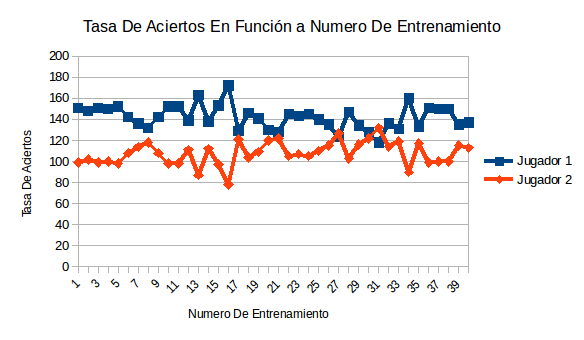
\includegraphics[scale=0.5]{testing/qvsq2.png}

La hipótesis parece confirmarse dado que el primer jugador obtiene un $20 \%$ mas de partidas ganadas que el segundo.

\subsection{Performance al cambiar la inicialización de Q}

En esta sección buscaremos ver que sucede al variar entre distintos valores iniciales la matriz de Q. Para ello utilizaremos un jugador random y un jugador q learning con estrategia greedy y variaremos Q. Como primer experimento cambiaremos el valor inicial de $1$ a $0$. De esta manera esperamos desalentar la fase de exploración del algoritmo y que se guíe en mayor grado por el camino óptimo encontrado hasta el momento. Los resultados fueron:

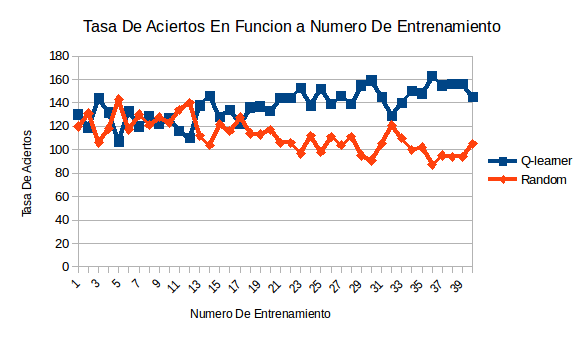
\includegraphics[scale=0.5]{testing/variarq.png}

Los resultados no parecen ser muy afectados por esta variación. Otra alternativa intermedia que ideamos podría ser iniciar los valores de Q con valores aleatorios en un rango definido de esa manera randomizando un poco mas que caminos son explorados y cuales no. En el siguiente experimento la matriz Q esta inicializada de con distribución uniforme en el rango $[-1,1]$:

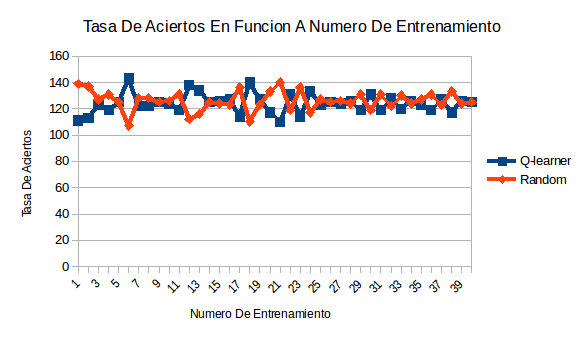
\includegraphics[scale=0.5]{testing/variarq2.png}

Como puede verse este tipo de exploración resulto en resultados muy malos, introducidos posiblemente por la dificultad de elegir un buen camino introduciendo un valor tan alto de ruido en el Q inicial.